\documentclass[11pt, a4paper]{article}
\usepackage[utf8]{inputenc}
\usepackage[left=2.35cm, right=3.35cm, top=3.35cm, bottom=3.0cm]{geometry}
\usepackage{amsmath, amssymb, amsthm}
\usepackage[english]{babel}
\usepackage{graphicx}
\usepackage[font={small,it}]{caption}
\graphicspath{ {figures/} }
\usepackage{url}
\usepackage{appendix}
\usepackage{float}
\usepackage[bottom]{footmisc}
\usepackage{titling}

\begin{document}

\begin{titlepage}
  \begin{center}
    
    
\includegraphics[scale=1.5]{figures/kuleuven_logo.pdf}~\\[4.5cm]
    \textsc{\Large Master of bioinformatics}\\[0.5cm]

    % Title
    \rule{\linewidth}{0.3mm}\\[0.4cm]
    {\huge \bfseries Support Vector Machines} \\[0.4cm]
    {\large Assignment 1: Classification} \\[0.4cm]
    \rule{\linewidth}{0.3mm}\\[0.4cm]
    {\large Spring 2016} \\[1.0cm]
    
    % Author and supervisor
    \begin{minipage}{0.4\textwidth}
      \begin{flushleft} \large
        \emph{Author:}\\
	Cedric \textsc{Lood}
      \end{flushleft}
    \end{minipage}
%     %\hfill
    \begin{minipage}{0.4\textwidth}
      \begin{flushright} \large
        \emph{Supervisors:} \\
        Dr. Carlos \textsc{Alaiz}\\
        Dr. Emanuele \textsc{Frandi}\\
        Prof. Johan \textsc{Suykens}\\
        \hfill \newline 
      \end{flushright}
    \end{minipage}
    
    \vfill

    
\includegraphics[scale=0.15]{figures/KUL.jpg}~\\[0.5cm]

    % Bottom of the page
    {\large \today}
    
  \end{center}
\end{titlepage}

\tableofcontents
\newpage

\section*{Context}

The analysis presented in this report was produced for the class of
``Support Vector Machines: methods and applications'' (Spring 2016) at
KU Leuven. The goal is to display understanding of the techniques and
of their practical use. This first report focuses on classification
using SVM, and Least-Squares SVM (LS-SVM). The implementation was done
using the MatLab software (v2015a) and the libraries for LS-SVM
developed at KU Leuven.

\section{Two Gaussians}

In this first application, an artificial dataset was generated
consisting of 100 points in $\mathbb{R}^2$. Two centroids were defined
to generate the points, one at $(1,1)$ and the other at $(-1,-1)$. For
both centers, 50 datapoints were generated by adding a gaussian noise
$N(0,1)$. Since we know the true underlying distribution for both
classes, we can define an optimal classifier as per the Bayesian
Decision Theory. This classifier, regardless of the overlap between
the distributions of the 2 classes, will consist of a line in
$\mathbb{R}^2$, and otherwise a hyperplane in higher dimensions.

\begin{figure}[H]
    \centering
    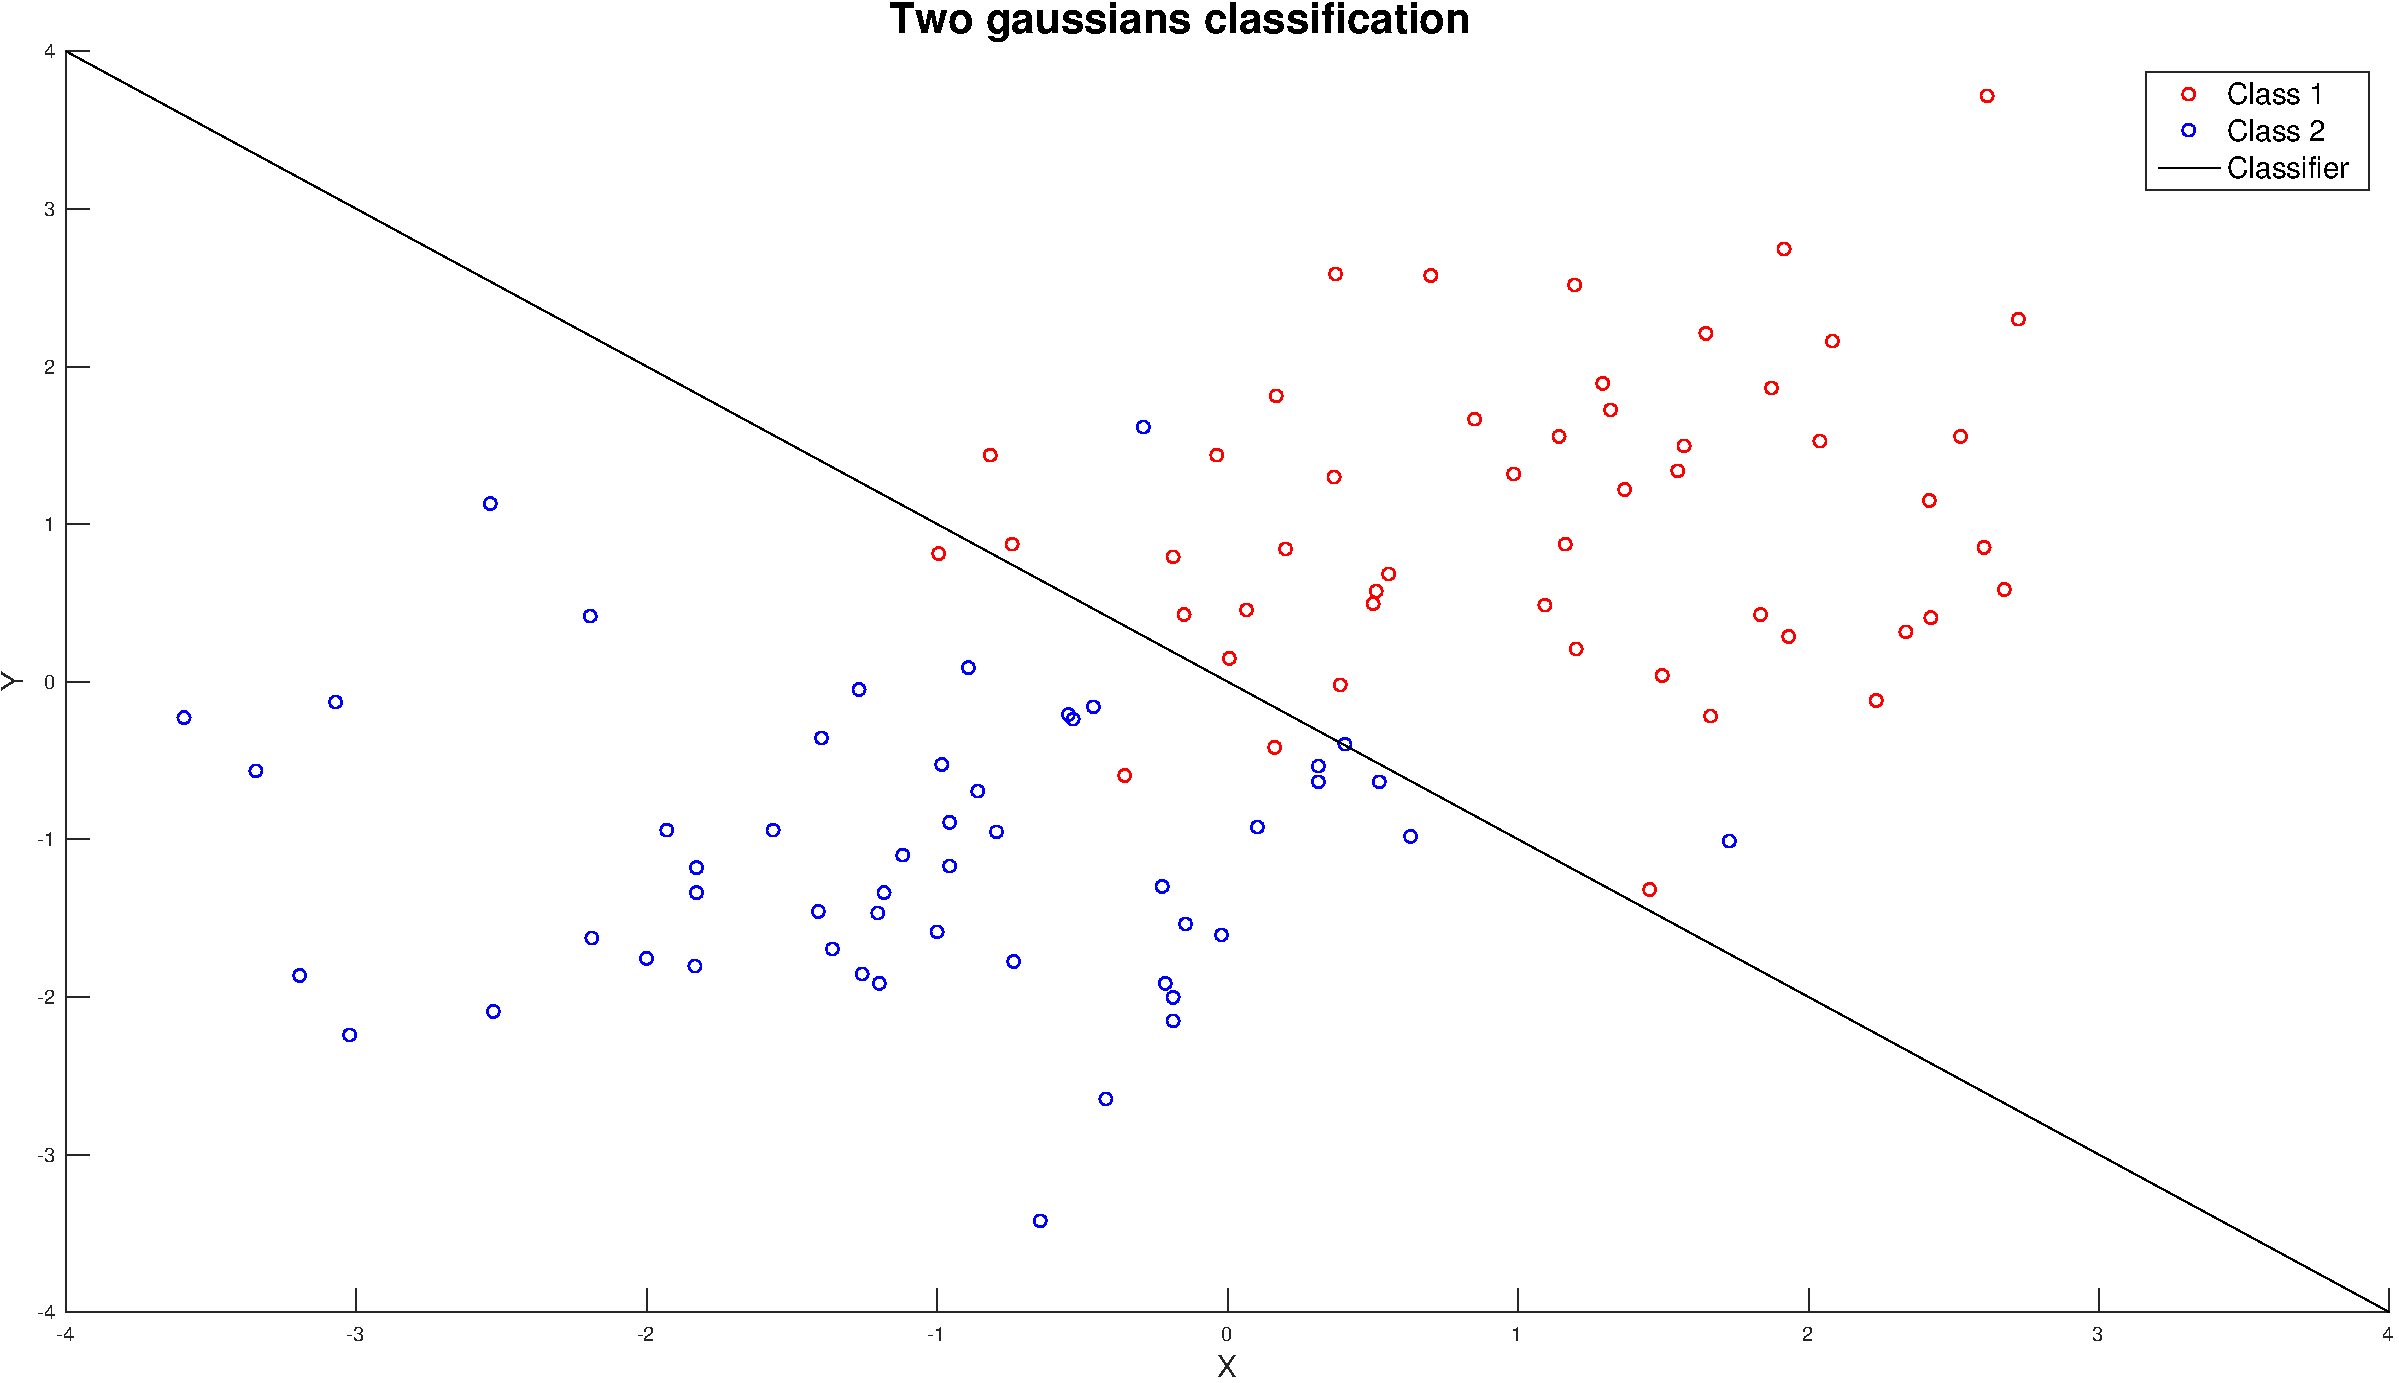
\includegraphics[scale=.40]{two_gaussians.pdf}
    %\caption{Two gaussians classification}
    \label{fig:two_gaussians}
\end{figure}

\section{Support Vector Machine}

The exercises in this section consisted of exploring the properties of
Support Vector Machines via a web application
\footnote{http://cs.stanford.edu/people/karpathy/svmjs/demo/}

\subsection{Linear kernel (q1,q2,q3)}
\subsection{RBF kernel (q4,q5)}
\subsection{Other (q6,q7,q8)}

\section{Least-Squares Support Vector Machine}

\section{Applications} 

\bibliographystyle{ieeetr} \bibliography{bib-db}
\end{document}
